\documentclass[a4paper,11pt,twoside]{book}

\usepackage{palatino,newtxmath,bbold}	%% Písma
\usepackage{microtype}					%% Lepší mezery
\usepackage[T1]{fontenc}
\usepackage[utf8]{inputenc}	            %% Kódování textu
\usepackage[czech]{babel}               %% České nápisy
\usepackage{amsfonts,amsmath}			%% Matematické symboly (amssymb koliduje s jiným balíkem)

\usepackage{epsfig}                     %% Obrázky
\usepackage[subrefformat=simple,labelformat=simple]{subcaption} %% Podobrázky
\usepackage{graphicx}					%% Doplňující příkazy pro obrázky

\usepackage{xifthen}					%% Podmínka if - then
\usepackage{makeidx}					%% Rejstřík
%\usepackage{showframe}
%\usepackage{showidx}

\usepackage[multiple]{footmisc}			%% Lepší formátování poznámek pod čarou - nefunguje s hyperref
%\usepackage{fnpct}						%% Lepší formátování poznámek pod čarou
\usepackage{comment}					%% Komentáře
\usepackage{scrextend}					%% Vylepšené formátování (addmargin)
\usepackage{xcolor}						%% Barvy
\usepackage{indentfirst}				%% Odsazení prvního odstavce
\usepackage{fancyhdr}
\usepackage{blkarray}					%% Pro komentované vektory
\usepackage{empheq}                     %% Box around equations

\usepackage{csquotes}

\graphicspath{{figures/}}

\usepackage{mathtools}

\usepackage[unicode]{hyperref}			%% Hypertextové odkazy
\hypersetup{
	pdftitle={Cvičení ke cvičení Kvantová teorie},
	pdfauthor={Pavel Stránský},
	pdffitwindow=true,
	colorlinks=true,
	urlcolor=cyan,            			%barva textu pri tisku
	linkcolor=red,
	citecolor=green,
	filecolor=magenta
}

\usepackage[sorting=none,style=phys]{biblatex}
\addbibresource{S:/Fyzika/Bibliography/References.bib}
\addbibresource{References.bib}

% Velikost stránky
\addtolength{\topmargin}{-2.2cm} %\addtolength{\textheight}{-10cm}
\addtolength{\leftmargin}{-2cm}
\addtolength{\textwidth}{4cm} \addtolength{\textheight}{4.5cm} % Šířka a výška textu
\setlength{\headheight}{15pt}
\setlength{\headsep}{0.5cm}

\addtolength{\oddsidemargin}{-2cm}
\addtolength{\evensidemargin}{-2cm}

\pagestyle{empty}

\input{LaTeX_defs/defs}

\def\np{\newpage}

\newenvironment{note}[1][]{\vspace*{0.2cm}\noindent\textbf{\textit{\ifthenelse{\isempty{#1}}{Poznámka: }{#1}}}}{}

\newcommand{\exercise}[2][]{\ifthenelse{\isempty{#1}}
	{\np\section{#2}}
	{\np\section{#2}\small{\it{(termín odevzdání: {#1})}\newline}}
}

\begin{document}
\makeatletter
\@addtoreset{equation}{subsection}

\renewcommand{\thechapter}{}
\renewcommand{\thesection}{\arabic{section}}

\title{Domácí úkoly k přednášce Kvantová teorie}
\date{\today}
\author{Pavel Stránský}
\makeatother

\maketitle
\pdfbookmark{\contentsname}{Contents}
\tableofcontents

\chapter{2023 -- 2024}
\exercise{BCH formule}
    Jsou dány dva nekomutující operátory $\operator{M}$, $\operator{N}$, které komutují se svým komutátorem:
    \begin{equation*}
        \commutator{\operator{M}}{\commutator{\operator{M}}{\operator{N}}}
            =\commutator{\operator{N}}{\commutator{\operator{M}}{\operator{N}}}
            =0.
    \end{equation*}
    Nalezněte, čemu se rovnají operátory $\operator{X}$, $\operator{Y}$ ve výrazech
    \begin{equation*}
    \e^{\operator{M}}\e^{\operator{N}}
        =\e^{\operator{M}+\operator{N}}\e^{\operator{X}}
        =\e^{\operator{X}}\e^{\operator{M}+\operator{N}}
        =\e^{\operator{M}+\operator{N}+\operator{Y}}
    \end{equation*}
    a dokažte, že platí všechny uvedené rovnosti.

    \emph{Nápověda:} 
        Nadefinujte a použijte funkci $\operator{g}(\xi)\equiv\e^{\xi\operator{M}}\e^{\xi\operator{N}}$.
        Využijte výsledků příkladů ze cvičení.

    \emph{Poznámka:} 
        Tento vztah se nazývá \emph{Baker-Campbell-Hausdorffova formule} nebo \emph{Glauberova formule}.

\exercise{Jednoduché kvantové systémy}
    \subsection{Kvantový řetízek}    
        Určete vlastní hodnoty a normalizované vlastní vektory Hamiltoniánu dimenze $N$ ve tvaru tridiagonální matice    
        \begin{equation*}
            \matrix{H}
                =\makematrix{e & v & 0 & 0 & \\ v & e & v & 0 & \\ 0 & v & e & v & \ldots 
                    \\ 0 & 0 & v & e & \\ & & \vdots & & \ddots}.
        \end{equation*}
        Jak se bude měnit energetické spektrum s rostoucím $N$?
    
        \begin{note}[Nápověda:]
            V charakteristické rovnici identifikujte diferenční rovnici pro složky $c_{k}, k=1,\cdots,n$ vlastních vektorů a řešte ji pomocí násady $c_{k}=u^{k}$.
        \end{note}
    
        \begin{note}
            Tento Hamiltonián popisuje například částici na řetízku délky $N$, která smí \uv{přeskočit} jen na sousední pozice:
            \begin{equation*}
                \operator{H}=e\sum_{k=1}^{N}\ket{k}\bra{k}+v\sum_{n=1}^{N-1}\left(\ket{k}\bra{k+1}+\ket{k+1}\bra{k}\right),
            \end{equation*}
            kde $\left\{\ket{k},k=1,\dotsc,N\right\}$ je ortonormální báze.
            V případě, kdy $N$ je velké, se jedná o jednoduchý model jednorozměrného krystalu.
        \end{note}
    
    \subsection{Kvantový oblak}
        Určete vlastní hodnoty a normalizované ortogonální vlastní vektory Hamiltoniánu dimenze $N$ daného maticí
        \begin{equation*}
            \matrix{H}
                =\makematrix{e & v & v & v & \\ v & e & v & v & \\ v & v & e & v & \ldots 
                    \\ v & v & v & e & \\ & & \vdots & & \ddots}.
        \end{equation*}
        Tento Hamiltonián popisuje například částici na mřížce o $N$ pozicích, přičemž částice může přeskočit na libovolnou pozici mřížky a žádná pozice není upřednostněna.

\exercise{Interakce spinu s dvouhladinovým systémem}
    Částice se spinem $\frac{1}{2}$ interaguje s dvoustavovým systémem tak, že výsledný stavový vektor systému je ve stavu
    \begin{equation*}
        \ket{\psi}=\alpha\left(\ket{\uparrow}+\ket{\downarrow}\right)\otimes\ket{0}+\beta\left(\ket{\uparrow}-\ket{\downarrow}\right)\otimes\ket{1},
    \end{equation*}
    kde $\ket{\uparrow},\ket{\downarrow}$ jsou ortonormální bázové vektory Hilbertova prostoru $\hilbert{H}_{s}$ spinu, které odpovídají projekci spinu podél souřadné osy $z$ a proti souřadné ose $z$, a $\left\{\ket{0},\ket{1}\right\}$ je ortonormální báze Hilbertova prostoru $\hilbert{H}_{2}$ dvoustavového systému.

    \begin{enumerate}
        \item
            Nalezněte podmínku pro komplexní parametry $\alpha,\beta\in\mathbb{C}$, aby stav $\ket{\psi}$ byl normalizovaný.

        \item
            Určete, jestli je stav $\ket{\psi}$ provázaný nebo faktorizovaný.

        \item
            Předpokládejte, že měříte projekci spinu částice do směru daného jednotkovým vektorem $\vector{n}$, který svírá s osou $z$ úhel $\theta=\frac{\pi}{3}$ a leží v rovině $xz$.
            Nalezněte projekční operátory odpovídající tomuto měření a pro každý možný výsledek měření určete pravděpodobnost jeho nalezení a stavový vektor složeného systému po měření.
    \end{enumerate}

\exercise{Kvartický oscilátor}
    \begin{enumerate}
    \item
        V jednorozměrném harmonickém oscilátoru popsaném Hamiltoniánem
        \begin{equation*}
            \operator{H}_{0}=\frac{1}{2M}\operator{p}^{2}+\frac{1}{2}M\Omega^{2}\operator{x}^{2}
        \end{equation*}
        vyjádřete maticové elementy
        \begin{align*}
        &\matrixelement{m}{\operator{x}^{2}}{n}\,,\\
        &\matrixelement{m}{\operator{x}^{4}}{n}\,,
        \end{align*}
        kde $\ket{m}$ a $\ket{n}$ jsou dva libovolné vlastní vektory Hamiltoniánu $\operator{H}_{0}$.
        
    \item
        Uvažujte Hamiltonián
        \begin{equation*}
            \operator{H}=\frac{1}{2M}\operator{p}^{2}+\frac{1}{2}M\Omega^{2}\operator{x}^{2}+\frac{1}{8}b\operator{x}^{4}
                =\operator{H}_{0}+\frac{1}{8}b\operator{x}^{4}\,,
        \end{equation*}
        kde $b$ je reálný kladný parametr.
        
        \begin{itemize}
        \item
            Napočítejte maticové elementy $H_{mn}=\matrixelement{m}{\operator{H}}{n}$ pro $M=\Omega=\hbar=1,b=10$
            a numerickou diagonalizací matice $\matrix{H}=\left(H_{mn}\right)$ 
            (například pomocí programů Mathematica, Maple, Matlab, GNU Octave, Python, Julia, knihoven LAPACK, atd.) 
            učete energie základního stavu $E_{0}$ a prvních tří vzbuzených stavů $E_{1,2,3}$ Hamiltoniánu $\operator{H}$.
            Uvažujte pouze konečný počet $N$ elementů báze, tj. $m,n=0,1,\dotsc,N-1$.

        \item 
            Zakreslete graf závislosti $E_{j}(N)$, $j=0,1,2,3$ pro $N\leq50$.

        \item
            Na základě výsledků z předchozího bodu odhadněte, jaká musí být nejmenší velikost matice $N$, aby čtyři nejnižší energie byly určeny s přesností na pět platných cifer.
        \end{itemize}
        
    \item
        Uvažujte nyní Hamiltonián
        \begin{equation*}
            \operator{H}'=\frac{1}{2M}\operator{p}^{2}-\frac{1}{2}a\operator{x}^{2}+\frac{1}{8}b\operator{x}^{4}\,,
        \end{equation*}
        kde $a>0$, $b>0$.
        
        \begin{itemize}
        \item 
            Načtněte klasický potenciál
            \begin{equation*}
                V(x)=-\frac{1}{2}ax^{2}+\frac{1}{8}bx^{4}
            \end{equation*}
            pro $a=b=1$ a nalezněte jeho stacionární body.
        \item 
            Vypočítejte numericky první čtyři energetické hladiny pro $\hbar=0.2,M=a=b=1$.
            Velikost matice ať je taková, aby tyto hladiny byly určeny s přesností alespoň na pět platných cifer.
        \item 
            Proč jsou dvojice hladin $(E_{0}, E_{1})$ a $(E_{2}, E_{3})$ v téměř degenerovaných dubletech?        
        \item 
            Opakujte výpočet pro jiné hodnoty $\hbar$, například $\hbar=0.1$ a $\hbar=0.5$, a diskutujte, jaký vliv má volba $\hbar$ na výsledné spektrum.
            Nezapomeňte pokaždé zkontrolovat konvergenci energetických hladin (obecně pro menší hodnoty $\hbar$ je potřeba více bázových stavů).
        \end{itemize}		
        
        \emph{Poznámka:} Dvoujámový systém popsaný Hamiltoniánem $\operator{H}'$ se požívá například k modelování amoniakového maseru, k modelování systémů ochlazených iontů, v teorii kvantové informace, při studiu kvantových fázových přechodů nebo v kvantové chemii.
            
    \end{enumerate}

\exercise{Kvantový míček}
    Částice o hmotnosti $M$ (míček) skáče v homogenním (např. gravitačním) poli, přičemž od podložky se odráží bez ztráty energie.
    Potenciál se tedy dá vyjádřit jako
    \begin{equation*}
        V(z)=
        \begin{cases}
        Mgz & z > 0, \\
        \infty & z < 0,
        \end{cases}
    \end{equation*}
    kde $z$ je svislá souřadnice a $g$ konstanta úměrnosti (gravitační zrychlení).

    Hledejte variační metodou přibližnou energii základního stavu a odpovídající vlastní funkci v $x$-reprezentaci.
    \begin{enumerate}
        \item 
            Podle vlastností potenciálu navrhněte vhodnou testovací funkci s jedním parametrem a správnými okrajovými podmínkami (dodatečný multiplikativní parametr bude fixovat normalizaci).

        \item 
            Nalezněte optimální hodnotu parametru a jemu odpovídající přibližnou energii základního stavu.

        \item 
            \emph{(volitelné)} Vyzkoušejte ještě jinou testovací funkci a rozhodněte, která přesněji aproximuje základní stav.
    \end{enumerate}	

\exercise{Moment hybnosti atomu vodíku}
    Jádro atomu vodíku (proton) má spin $s_{p}=\frac{1}{2}$, spin obíhajícího elektronu je $s_{e}=\frac{1}{2}$ a elektron se nachází na orbitalu $d$ (velikost orbitálního moment hybnosti je tedy $l=2$).
    Operátor celkového momentu hybnosti je
    \begin{equation*}
        \vectoroperator{J}=\vectoroperator{S}^{(p)}+\vectoroperator{S}^{(e)}+\vectoroperator{L}.
    \end{equation*}
    
    \begin{enumerate}
    \item
        Určete celkový počet odlišných kvantových stavů, kterých může moment hybnosti $\vectoroperator{J}$ nabývat.
        
    \item
        Určete, jaké hodnoty může mít celkový moment hybnosti $j$ a kolik stavů přísluší každé jeho hodnotě.
        
    \item
        Určete normalizované stavy
        \begin{equation*}
            \ket{j\,m}=\begin{cases}\ket{3\,3} \\ \ket{3\,2} \\ \ket{3\,1} \\ \ket{3\,0}\end{cases},
        \end{equation*}
        kde $m$ značí projekci celkového momentu hybnosti $\vectoroperator{J}$ na třetí souřadnou osu.
        
    \item
        Určete střední hodnotu
        \begin{equation*}
            \matrixelement{3\,2}{\vectoroperator{S}^{(e)}\cdot\vectoroperator{S}^{(p)}}{3\,2}\,.
        \end{equation*}

\emph{Nápověda:}
    Skalární součin operátorů $\vectoroperator{S}^{(e)}\cdot\vectoroperator{S}^{(p)}$ vyjádřete pomocí
    operátorů $\operator{S}^{(e,p)}_{\pm}$ a $\operator{S}^{(e,p)}_{3}$.	
    \end{enumerate}

\exercise{Dvě $\delta$ jámy nebo bariéry}
    Částice o hmotnosti $M$ se pohybuje v potenciálu složeném ze dvou $\delta$ funkcí vzdálených od sebe o délku $d$,
    \begin{equation*}
        V(x)=c\left[\delta\left(x-\frac{d}{2}\right)+\delta\left(x+\frac{d}{2}\right)\right].
    \end{equation*}
    
    \begin{enumerate}
    \item
        Nalezněte rovnici pro vázané stavy systému ($E<0$, $c<0$) a vyřešte ji numericky.
        Porovnejte výsledné energetické spektrum s případem jedné jámy.
        
    \item
        Pro $E>0$ určete pravděpodobnost průchodu $T(E)$ a pravděpodobnost odrazu $R(E)$.
        Zakreslete $T(E)$ do grafu společně s pravděpodobností průchodu skrz jednu $\delta$ funkci.
        
    % \item
    %     Pro $E>0$ určete fázové posunutí $\delta(E)$.
    %     Zakreslete fázové posunutí do grafu společně s fázovým posunutím pro jednu $\delta$ funkci.
    \end{enumerate}
    
    Pro všechny číselné výpočty uvažujte $\hbar=M=\abs{c}=d=1$.
        
\exercise{Diracův hřeben}
    Částice se pohybuje v potenciálu složeném z periodicky se opakujících $\delta$ funkcí
    \begin{equation*}
        V(x)=c\sum_{n=-\infty}^{\infty}\delta(x-na),
    \end{equation*}
    jehož vlnové funkce na intervalu 
    $x\in\left(na; \left(n+1\right)a\right)$, $n\in\mathbb{Z}$, $E>0$ 
    jsou podle Blochova teorému
    \begin{equation*}
        \psi_{q}(x)
            =\left[A\e^{\im k\left(x-na\right)}+B\e^{-\im k\left(x-na\right)}\right]\e^{iqna},
    \end{equation*}
    kde $q$ je krystalová hybnost (kvazihybnost) částice.
    Mezi $k=\sqrt{2ME}/\hbar$ a $K$ platí vztah
    \begin{equation*}
        \cos{qa}=\cos{ka}+\frac{K}{2k}\sin{ka},
    \end{equation*}
    kde $K=2Mc/\hbar^{2}$ ($M$ je hmotnost částice).
    \begin{enumerate}
    \item 
        Pro dvě hodnoty $K=2$ a $K=10$ vypočítejte a na počítači vykreslete graf disperzní relace $E(q)$ pro nejnižší čtyři energetické pásy.
        Uvažujte následující konvenci: pokud $\pi n\leq ka\leq\pi(n+1)$, pak $\pi n\leq qa\leq\pi(n+1)$, $n\in\mathbb{Z}$.
    \item 
        Vypočítejte grupovou rychlost
        \begin{equation*}
            v_{\ti{g}}=\frac{1}{\hbar}\frac{\partial E}{\partial q}
        \end{equation*}
        a zakreslete její závislost na $q$ a na $E$ pro dvě hodnoty parametru $K=2$, $K=10$ a nejnižší čtyři energetické pásy.
        Srovnejte s případem volné částice.
    \item
        Najděte řešení Schrödingerovy rovnice pro případ $K<0$ (v tomto případě může být energie i záporná, $E<0$).
        Podobně jako v bodě 1 zakreslete disperzní relaci $E(q)$ pro $K=-2$ a $K=-10$.

    % \item 
    % 	Nalezněte parametry $A$, $B$ vlnové funkce. Vlnovou funkci normalizujte na intervalu mezi sousedními dvěma $\delta$ funkcemi:
    % 	\begin{equation*}
    % 		\label{eq:psiqnorm}
    % 		\int_{0}^{a}\abs{\psi_{q}(x)}^{2}\d x=1.
    % 	\end{equation*}
    \end{enumerate}

    Pro všechny numerické výpočty uvažujte $a=M=\hbar=1$.

\exercise{Koherentní stavy v $x$-reprezentaci}
    \begin{enumerate}
    \item 
        Vyjádřete vlnovou funkci $\psi_{z}(x)\equiv\braket{x}{z}$ koherentního stavu harmonického oscilátoru v $x$-reprezentaci.
        Využijte toho, že koherentní stav je vlastním stavem snižovacího operátoru~$\operator{a}$,
        \begin{equation*}
            \operator{a}\ket{z}=z\ket{z},
        \end{equation*}
        a operátor $\operator{a}$ vyjádřete pomocí operátorů souřadnice $\operator{x}$ a hybnosti $\operator{p}$ v $x$-reprezentaci.
        Vyřešte vzniklou diferenciální rovnici pro $\psi_{z}(x)$.

    \item Vlnovou funkci $\psi_{z}(x)$ nanormujte.

    \item 
        Dosaďte 
        \begin{equation*}
            z=\sqrt{\frac{M\Omega}{2\hbar}}\left(\langle\operator{x}_{z}\rangle+\frac{\im}{M\Omega}\langle\operator{p}_{z}\rangle\right)
        \end{equation*}
        a dokažte, že hustota pravděpodobnosti $|\psi_{z}(x)|^{2}$ nalezení částice v bodě $x$ odpovídá Gaussovskému vlnovému balíku.
        Určete jeho disperzi $\sigma$.

    \item 
        Určete hustotu pravděpodobnosti $\abs{\psi_{z}(x;t)}^2$ v čase $t$.
        Dokažte, že se stále bude jednat o gaussovský vlnový balík, jehož disperze $\sigma$ se s časem nemění (vlnový balík se nerozplývá) a jehož střední hodnota kmitá okolo počátku s klasickou frekvencí harmonického oscilátoru $\Omega$.
        
    \item
        Vyjádřete normalizovanou vlnovou funkci $\tilde{\psi}_{z}(p;t)\equiv\braket{p}{z(t)}$ v $p$-reprezentaci.

    \end{enumerate}

\exercise{Ramseyův přístroj pro spin 1}
    Částice se spinem $1$ a velikostí magnetického momentu $\mu$, popsaná vlnovou funkcí
    \begin{equation*}
        \ket{\psi(t)}=\psi_{+1}(t)\ket{+1}+\psi_{0}(t)\ket{0}+\psi_{-1}(t)\ket{-1}=\makematrix{\psi_{+1}(t) \\ \psi_{0}(t) \\ \psi_{-1}(t)},
    \end{equation*}
    kde dolní index určuje projekci spinu na osu $z$,
    se pohybuje v zařízení složeném ze tří oblastí.
    V~první oblasti (1. Ramseyova oblast) je zapnuté magnetické pole složené ze stacionární složky $\vector{B}_{0}$ směřující podél osy $z$ 
    a rotující složky $\vector{B}_{1}(t)$ v rovině $(x,y)$,
    \begin{align*}
        \vector{B}_{0}&=(0,0,B_{0}),&
        \vector{B}_{1}(t)&=(B_{1}\cos{\omega t},-B_{1}\sin{\omega t},0),
    \end{align*}
    a částice v ní stráví dobu dobu $\tau$.
    V druhé oblasti je rotující pole vypnuto a po dobu $T$ se částice pohybuje pouze ve stacionárním poli $\vector{B}_{0}$.
    Poté (2. Ramseyova oblast) je rotující pole zapnuto, a to opět na dobu $\tau$.
    
    \begin{enumerate}
    \item
        Matice generující rotace částice se spinem $1$ jsou $\matrix{S}_{j}^{(1)}=\hbar\matrix{s}_{j}$, kde
        \begin{align*}
            \matrix{s}_{1}&=\frac{1}{\sqrt{2}}\makematrix{0 & 1 & 0 \\ 1 & 0 & 1 \\ 0 & 1 & 0}\,, &
            \matrix{s}_{2}&=\frac{1}{\sqrt{2}}\makematrix{0 & -\im & 0 \\ \im & 0 & -\im \\ 0 & \im & 0}\,, &
            \matrix{s}_{3}&=\makematrix{1 & 0 & 0 \\ 0 & 0 & 0 \\ 0 & 0 & -1}\,.
        \end{align*}
        Ukažte, že tyto matice splňují komutační relace pro moment hybnosti
        \begin{equation*}
            \commutator{\matrix{s}_{j}}{\matrix{s}_{k}}=\im\epsilon_{jkl}\matrix{s}_{l}\,.
        \end{equation*}
        (Matice $\matrix{s}_{j}$ jsou analogické k Pauliho maticím $\matrix{\sigma}_{j}$ popisujícím částici se spinem $1/2$ a tvoří generátory třírozměrné ireducibilní reprezentace grupy $\group{SU}(2)$.)
        
    \item
        Dokažte, že pro matice $\matrix{s}_{j}$ platí $\matrix{s}_{j}^{n+2}=\matrix{s}_{j}^{n}$, 
        kde $n\in\mathbb{N}$, a na základě tohoto vztahu vyjádřete exponenciálu
        \begin{equation*}
            \e^{\im\phi\left(\vector{\hat{n}}\cdot\vector{\matrix{s}}\right)}=?
        \end{equation*}
        kde $\vector{\hat{n}}$ je jednotkový vektor určující osu rotace, okolo které se systém otočí o úhel $\phi$, a
        \begin{equation*}
            \vector{\hat{n}}\cdot\vector{\matrix{s}}\equiv\hat{n}_{1}\matrix{s}_{1}+\hat{n}_{2}\matrix{s}_{2}+\hat{n}_{3}\matrix{s}_{3}\,.
        \end{equation*}
        
    \item
        Vyjádřete složky evolučního operátoru
        \begin{equation*}
            \matrix{U}(t)=\e^{\im\omega t\matrix{s}_{3}}\e^{-\im\Omega t\left(\vector{\hat{n}}_{\Omega}\cdot\vector{\matrix{s}}\right)},
        \end{equation*}
        kde
        \begin{align*}
            \Omega&=\sqrt{(\omega-\omega_{0})^{2}+\omega_{1}^{2}}\,, &
            \vector{\hat{n}}_{\Omega}&=\frac{1}{\Omega}\makematrix{-\omega_{1} \\ 0 \\ \omega-\omega_{0}}\,, &
            \omega_{0,1}&=\frac{2\mu}{\hbar}B_{0,1}\,.
        \end{align*}
        
    \item
        Vyjádřete složky evolučního operátoru $\matrix{U}(t;t_{0})$, který vyvíjí systém z času $t_{0}$ do času $t$.
        
    \item
        Vyjádřete složky evolučního operátoru $\matrix{U}_{0}(\tau+T;\tau)$ oblasti, kde je vypnuté pole $\vector{B}_{1}$.
            
    \item
        Proces průchodu zařízením složeným z dvou Ramseyových oblastí s mezioblastí s vypnutým polem $B_{1}$ je dán evolučním operátorem
        \begin{equation*}
            \matrix{U}_{F}=\matrix{U}(2\tau+T;\tau+T)\matrix{U}_{0}(\tau+T;\tau)\matrix{U}(\tau;0)\,.
        \end{equation*}
        Vyjádřete složky evolučního operátoru $\matrix{U}_{F}^{\ti{rez}}$ pro speciální případ $\omega=\omega_{0}$ (frekvence oscilujícího magnetického pole $\vector{B}_{1}$ je v rezonanci s Larmorovou frekvencí $\omega_{0}$).
        
    \item
        Vypočítejte matici $\matrix{p}^{\ti{rez}}$ se složkami $p^{\ti{rez}}_{fi}$,
        které udávají pravděpodobnosti, že systém připravený na před vstupem do přístroje ve stavu 
        s projekcí spinu na osu $z$ rovnou $i\in\{+1,0,-1\}$, 
        naměříme po průchodu zařízením ve stavu s projekcí spinu $f\in\{+1,0,-1\}$.
        Jaká podmínka musí být splněna, aby byla pravděpodobnost překlopení spinu největší?

    \end{enumerate}

\exercise{Isotopický posun energie}
    Hamiltonián elektronu pohybujícího se v blízkosti bodového atomového jádra se $Z$ protony má tvar
    \begin{equation*}
        \operator{H}_{0}=\frac{\vectoroperator{p}^{2}}{2m}-\frac{\gamma Z}{\operator{r}}\,,
    \end{equation*}	
    kde $m$ je hmotnost elektronu (předpokládáme, že je malá v porovnání s hmotností jádra), $\gamma=e^{2}/(4\pi\epsilon_{0})$, $e$ je elementární náboj a $\epsilon_{0}$ permitivita vakua.
    Předpokládáme dále, že atom je ionizovaný a v atomovém obalu se nachází pouze jeden elektron na nejnižším $1s$ stavu.
    Energie tohoto elektronu a odpovídající vlnová funkce jsou
    \begin{align*}
        E_{0}^{(0)}&=-\frac{mZ^{2}\gamma^{2}}{2\hbar^{2}}=-\frac{Z^{2}\gamma}{2a_{0}}\,,\\
        \psi_{0}(r,\theta,\phi)&=\frac{1}{\sqrt{\pi}}\left(\frac{Z}{a_{0}}\right)^{\frac{3}{2}}\e^{-\frac{Zr}{a_{0}}}\,,
    \end{align*}
    kde $a_{0}=\hbar^{2}/(\gamma m)$ je Bohrův poloměr.
    
    Ve skutečnosti však má jádro konečný poloměr, který lze v prvním přiblížení aproximovat vzorcem
    \begin{equation*}
        R=R_{0}\sqrt[3]{A}\,,
    \end{equation*}
    kde $R_{0}=1,\!2\,\mathrm{fm}$ a $A$ je atomové číslo (celkový počet nukleonů).
    
    Předpokládejte, že hustota elektrického náboje v jádře je konstantní.
    \begin{enumerate}
    \item
        Určete Hamiltonián $\operator{H}$ elektronu, který se pohybuje v okolí jádra konečného poloměru.
        Rozdíl mezi $\operator{H}$ a $\operator{H}_{0}$ uvažujte jako malou poruchu $\operator{H}_{\mathrm{I}}$.
        
    \item
        V prvním řádu poruchové teorie spočítejte opravu k energii základního stavu elektronu,
        způsobenou konečností poloměru atomového jádra.
        
    \item
        Vypočítejte číselnou hodnotu \emph{isotopického posunu} energie základního stavu mezi v přírodě pozorovaným nejtěžším $A=124$ a nejlehčím $A=112$ stabilním izotopem cínu (cín je prvek s největším množstvím stabilních izotopů).
    \end{enumerate}

\exercise{Zenonův jev pro Ramseyův přístroj}
    Částice se spinem $1/2$ a velikostí magnetického momentu $\mu$ připravená ve stavu $\ket{\psi_{i}}=\ket{+}$ (spin ve směru osy $z$) vlétá do Ramseyova přístroje
    sestávajícího se z $N$ Ramseyových zón.
    V každé zóně na ni působí působí magnetické pole složené ze stacionární složky $\vector{B}_{0}$ směřující podél osy $z$ 
    a rotující složky $\vector{B}_{1}(t)$ v rovině $(x,y)$
    \begin{align*}
        \vector{B}_{0}&=(0,0,B_{0})\\
        \vector{B}_{1}(t)&=(B_{1}\cos{\omega t},-B_{1}\sin{\omega t},0)
    \end{align*}
    a částice v ní stráví dobu dobu $\tau$.
    Mezi zónami je tzv. \emph{monitorovací oblast}, ve které je magnetické pole $\vector{B}_{1}$ vypnuté a místo toho je zapnuto monitorování
    pomocí dalšího spinu o velikosti $1/2$.
    Tento spin se z neutrální polohy
    \begin{equation*}
        \ket{\phi_{i}}=\frac{1}{2}\makematrix{1-\im \\ 1+\im}
    \end{equation*}
    po interakci s procházejícím spinem za působení Hamiltoniánu
    \begin{equation*}
        \matrix{H}_{0}'=\left\{
            \begin{array}{ll}
                -\mu B_{0}\matrix{\sigma}_{3}\otimes\left[\matrix{1}+\frac{\lambda}{2}\left(\matrix{1}-\matrix{\sigma}_{1}\right)\right]\,, &\tau\leq t<\tau+T_{0}\,, \\
                -\mu B_{0}\matrix{\sigma}_{3}\otimes\matrix{1}\,, & \tau+T_{0}\leq t<\tau+T\,,
            \end{array}\right.
    \end{equation*}
    [$\sigma_{1}$ je první Pauliho matice, $\lambda=\pi\hbar/(2\mu B_{0}T_{0})$] přepne do polohy $\ket{+}$ nebo $\ket{-}$ podle orientace prolétávajícího spinu, viz obrázek.
    V monitorovací oblasti stráví částice dobu $T$.
    Změřením orientace monitorovacích spinů můžeme určit, v které z Ramseyových zón se orientace prolétávajícího spinu překlopila.
    Magnetická pole jsou naladěna tak, že $\omega=\omega_{0}$, kde $\omega_{0}=2\mu B_{0}/\hbar$.

    \begin{figure}[!h]
        \begin{center}
            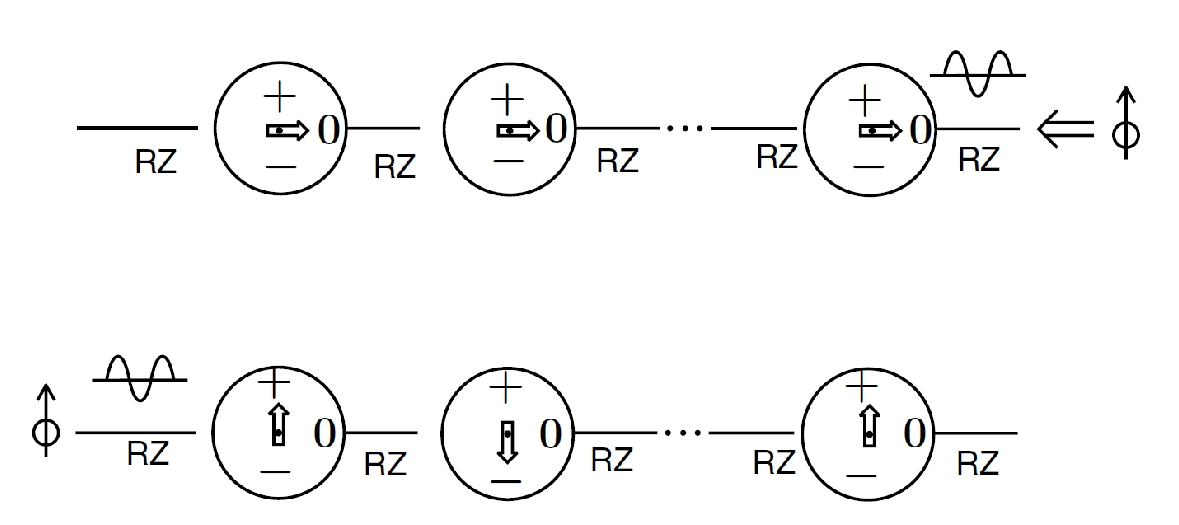
\epsfig{file=Ramsey.eps,width=0.8\linewidth}
        \end{center}
        \par{
            Obrázek: Schéma Ramseyova přístroje složeného z $N$ Ramseyových zón (RZ) se zapnutým oscilujícím polem, mezi kterými se nacházejí monitorovací oblasti znázorněné kružnicemi.
            Spin prochází přístrojem \emph{zprava doleva}. 
            Vpravo nahoře je zakreslena situace v čase $t=0$, vlevo dole dole v čase $t=N\tau+(N-1)T$.
        }
        \label{fig:ramsey}
    \end{figure}
    
    \begin{enumerate}
    \item
        Pro Ramseyův přístroj $N=2$ (tj. ten, který se počítal na cvičení) s vypnutým monitorováním ($\lambda=0$) nalezněte pravděpodobnost 
        $p^{(2)}_{(\uparrow\uparrow)}$, že spin vylétne ve stejném stavu, v jakém do přístroje vlétal (nepřeklopí se při průchodu přístrojem).
    
    \item
        Nalezněte pravděpodobnost $p^{(2)'}_{(\uparrow\uparrow)}$, že se spin nepřeklopí při zapnutém monitorování.
        Ukažte, že tato pravděpodobnost je vyšší než $p^{(2)}_{(\uparrow\uparrow)}$.
        
    \item
        Nalezněte pravděpodobnost $p^{(N)'}_{(\uparrow\uparrow)}$, že se spin nepřeklopí při zapnutém monitorování po
        průchodu $N$ Ramseyovými zónami.
        Využijte skutečnosti, že při zapnutém monitorování lze počítat s pravděpodobnostmi, že se spin překlopí nebo nepřeklopí v každé jednotlivé Ramseyově zóně, a že tyto pravděpodobnosti jsou pro všechny zóny stejné.

    \item
        Ukažte, že v limitě velkého množství malých kroků takových, aby doba průchodu přístrojem byla konstantní, tj. 
        \begin{equation*}
            \tau=\frac{\mathfrak{t}}{N},\quad T=\frac{\mathfrak{T}}{N},
        \end{equation*}
        platí 
        \begin{equation*}
            p^{(N)'}_{(\uparrow\uparrow)}\xrightarrow{N\rightarrow\infty}1.
        \end{equation*} 

        \emph{Poznámka}:
        Tento jev, kdy opakované měření zvyšuje pravděpodobnost přežití stavu, se nazývá \emph{kvantový Zenonův jev}.
        Poprvé ho zmínil již Alan Turing, obecné odvození rozpracovali A.~Degasperis, L.~Fonda a G.C.~Ghirardi (1974).%~\cite{Degasperis1974}.
    
    \item
        Nalezněte pravděpodobnost $p^{(N)}_{(\uparrow\uparrow)}$, že se spin nepřeklopí při vypnutém monitorování, a ukažte, že při zachování celkového času průletu přístrojem daného veličinami $\mathfrak{t},\mathfrak{T}$  tato pravděpodobnost nezávisí celkovém na počtu Ramseyových zón $N$.

        \emph{Nápověda:} Napočítejte matici evolučního operátoru pro $N=2$ a $N=3$ a \uv{uhodněte} její tvar pro obecné $N$.
    \end{enumerate}

\appendix
\chapter{Úkoly z dřívějších let}
\exercise{Hladká konečně hluboká potenciálová jáma}
    Částice o hmotnosti $M$ se pohybuje v jednorozměrném potenciálu
    \begin{equation*}
        V(x)=-\frac{V_{0}}{\cosh^{2}\frac{x}{a}}\,,
    \end{equation*}
    kde $a>0$ a $V_{0}>0$ jsou parametry udávající šířku a hloubku potenciálové jámy.
    Předpokládejte, že energie $E<0$, tj. uvažujte pouze vázané stavy.

    \begin{enumerate}
    \item
        Načrtněte potenciál.

    \item
        Schrödingerovu rovnici převeďte pomocí vhodných substitucí na rovnici pro 
        hypergeometrické funkce.
        
    \item
        Napište obě lineárně nezávislá řešení diferenciální rovnice.
        Za jakých podmínek budou tato řešení kvadraticky integrovatelná?
        Nalezněte kvantovací podmínky a energetické spektrum.
        
    \item
        Jaké podmínky musejí parametry $a$, $V_{0}$ a $M$ splňovat, 
        aby měl systém alespoň jeden vázaný stav?
        
    \item
        Kolik bude mít systém vázaných stavů pro $a=V_{0}=M=\hbar=1$?
        Napište jejich energie.
        
    \item
        \emph{(nepovinně)} Zakreslete vlnové funkce příslušející energiím z předchozího bodu. 
        Vlnové funkce nemusíte normalizovat.
    \end{enumerate}
    \emph{Nápověda:}
        Vlnovou funkci hledejte ve tvaru
        \begin{equation*}
            \psi(x)=u(x)\cosh^{\alpha}\frac{x}{a}\,,
        \end{equation*}
        kde $\alpha<0$.
        Zvolte vhodně tento parametr.
        Zaveďte nezávisle proměnnou
        \begin{equation*}
            z=-\sinh^{2}\frac{x}{a}\,.
        \end{equation*}	

\exercise{Interakce způsobená nerozlišitelností částic}
    Uvažujte dvě bezspinové volné nerozlišitelné částice o hmotnosti $M$ pohybující se na přímce.
    Jejich vlnové funkce jsou dány gaussovskými balíky dobře lokalizovanými okolo bodů $-b$ a $+b$ (obrázek),
    \begin{equation}
        \psi_{\pm}(x)=\frac{1}{\sqrt[4]{\pi\sigma^{2}}}\e^{-\frac{1}{2\sigma^{2}}(x\mp b)^{2}},
    \end{equation}
    kde $\sigma\ll b$ určuje určuje šířku balíku.
    
    \begin{figure}[htbp!]
        \centering
        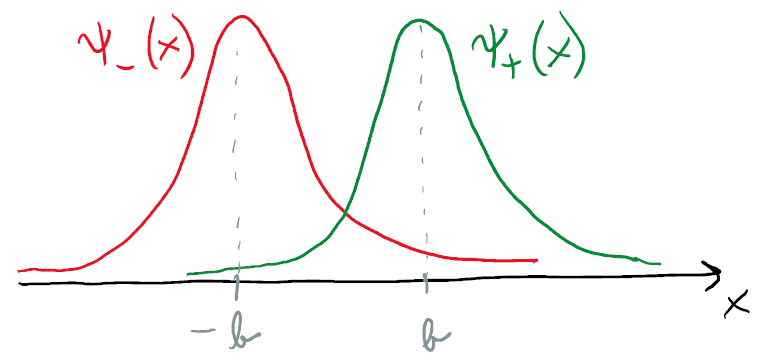
\includegraphics[width=0.5\linewidth]{Identical.png}
    \end{figure}

    \begin{enumerate}
        \item 
            Určete vlnovou funkci $\psi(x_{1},x_{2})$ systému těchto dvou nerozlišitelných částic a spočítejte její normalizaci.
            Částice mohou být bosony nebo fermiony. 
            Uvažujte oba dva případy.
        
        \item Spočítejte střední hodnotu energie systému dvou nerozlišitelných částic
            \begin{equation}
                E=\matrixelement{\psi}{\operator{H}}{\psi}=\int\psi^{*}(x_{1},x_{2})H\psi(x_{1},x_{2})\d x_{1}\d x_{2}.
            \end{equation}

        \item Spočítejte efektivní sílu
            \begin{equation}
                F\equiv-\frac{\partial E}{\partial b}.
            \end{equation}
            Bude tato síla přitažlivá nebo odpudivá a jak závisí na typu nerozlišitelných částic (bosony, fermiony)?
    \end{enumerate}

\exercise{Dvouhladinový systém s periodickou poruchou}
\label{sec:TwoLevelTD}
    Dvouhladinový systém je popsaný Hamiltoniánem
    \begin{align*}
        \operator{H}(t)
            &=\operator{H}_{0}+\operator{H}_{\ti{I}}(t),\\
        \operator{H}_{0}
            &=\makematrix{E_{1}^{\hi{0}} & 0 \\ 0 & E_{2}^{\hi{0}}}
                \equiv E_{1}^{\hi{0}}\ket{\phi_{1}}\bra{\phi_{1}}
                +E_{2}^{\hi{0}}\ket{\phi_{2}}\bra{\phi_{2}},\\
        \operator{H}_{\ti{I}}(t)
            &\equiv \Theta(t)\makematrix{0 & \gamma\e^{\im\omega t} \\ \gamma\e^{-\im\omega t} & 0}
                =\Theta(t)\left[\gamma\e^{\im\omega t}\ket{\phi_{1}}\bra{\phi_{2}}
                    +\gamma\e^{-\im\omega t}\ket{\phi_{2}}\bra{\phi_{1}}\right],
    \end{align*}
    přičemž operátor $\operator{H}_{\ti{I}}(t)$ představuje periodickou poruchu, která je zapnuta v čase $t_{0}=0$ (formálně zapsáno pomocí Heavisideovy skokové funkce $\Theta$), $\gamma$ je reálný parametr, který určuje sílu poruchy, a $E_{1,2}^{(0)}$ jsou neporušené energie.

    Před zapnutím poruchy v čase $t\leq0$ je systém ve stavu $\ket{\phi_{i}}\equiv\ket{\phi_{1}}=\makematrix{1\\0}$.

    \begin{enumerate}
    \item 
        Spočítejte neporuchově pravděpodobnost $\mathcal{P}_{1\rightarrow2}(t)$, že systém v čase v čase $t>0$ přejde do stavu $\ket{\phi_{2}}$.
        Vzorec, který dostanete, se nazývá \emph{Rabiho formule}.

        \item 
            Řešte totéž do druhého řádu nestacionární poruchové teorie a získanou pravděpodobnost srovnejte s přesným řešením.
            Za jaké podmínky toto přibližné řešení dobře aproximuje přesný výsledek?

        \item 
            Za jaké podmínky lze v čase $t>0$ naměřit systém ve stavu $\ket{\phi_{2}}$ s pravděpodobností jedna?
    \end{enumerate}
        
    \printbibliography

\exercise{Stimulovaná emise}
    Atom vodíku popsaný Hamiltoniánem
    \begin{equation*}
        \operator{H}_{0}
            =\frac{1}{2m}\vectoroperator{p}^{2}-\frac{\gamma}{\operator{r}},
    \end{equation*}
    se nachází v excitovaném stavu 2p, tj. ve stavu popsaném vektorem $\ket{n=2,l=1,m}$, kde projekce orbitálního momentu hybnosti $m$ může nabývat libovolné z hodnot $\{-1,0,1\}$.
    Na atom působí elektromagnetické vlnění s vektorovým potenciálem
    \begin{equation*}
        \vector{A}(\vectoroperator{r},t)
            =2A_{0}\vector{\epsilon}\cos\left(\vector{\kappa}\cdot\vectoroperator{r}-\omega t\right)
    \end{equation*}
    (jednotkový vektor $\vector{\epsilon}$ určuje polarizaci vln, $\vector{\kappa}=\vector{n}\omega/c$ je vlnový vektor určující směr postupu vlny)	a skalárním potenciálem
    \begin{equation*}
        \Phi(\vectoroperator{r},t)
            =0.
    \end{equation*}
    Předpokládejte, že vlnová délka $\lambda=2\pi/\kappa$ je mnohem větší než efektivní rozměr atomu $a_{0}$, lze tedy počítat v dipólové aproximaci.

    \begin{enumerate}
        \item Nalezněte hustotu pravděpodobnosti za jednotku času, že atom přejde do základního stavu a vyzáří foton o frekvenci $\omega$ do elementu prostorového úhlu $\Omega$.
        
        \item Napište diferenciální účinný průřez tohoto procesu.
        
        \item 
            Nalezněte směr polarizace $\vector{\epsilon}$ dopadajícího elektromagnetického vlnění, pro kterou je pravděpodobnost stimulované emise nejvyšší.
            Jak se se tento směr liší podle hodnoty kvantového čísla $m$ v počátečním stavu?
    \end{enumerate}      
        
\exercise{Rozptyl na $\frac{1}{r^{2}}$ potenciálu}
    Uvažujte rozptyl částice o hmotnosti $M$ na potenciálu
    \begin{equation*}
        V(r)=\frac{v}{r^{2}},
    \end{equation*}
    kde parametr $v$ může být kladný (pro odpudivou sílu) nebo záporný (pro sílu přitažlivou).
    
    \begin{itemize}
        \item 
            Řešením Schrödingerovy rovnice nalezněte vlnovou funkci pro energii $E>0$.
            
        \item
            Spočítejte fázové posunutí $\delta_{l}(k)$ $l$-té parciální vlny 
            a načrtněte jeho závislost na $k$ (nebo na energii $E$).
            
        \item
            Nalezněte totální účinný průřez pro $l$-tou parciální vlnu $\sigma_{l}(k)$.
            Diskutujte fyzikální příčinu skutečnosti, že pro $k\rightarrow0$ účinný průřez diverguje.
    \end{itemize}    

    \exercise[26.4.2022]{Magnetický moment}
	Dva nezávislé impulsmomenty $\vectoroperator{L}$ (například orbitální moment hybnosti) a $\vectoroperator{S}$ (vnitřní spin systému) splňující $\commutator{\vectoroperator{L}}{\vectoroperator{S}}=0$ se složí na celkový impulsmoment
	\begin{equation*}
		\vectoroperator{J}=\vectoroperator{L}+\vectoroperator{S}.
	\end{equation*}
	Stavem $\ket{(ls)jm}$ označme vlastní vektory operátorů $\vectoroperator{L}^{2}$, $\vectoroperator{S}^{2}$, $\vectoroperator{J}^{2}$, $\operator{J}_{3}$:
	\begin{align*}
		\vectoroperator{L}^{2}\ket{(ls)jm}&=l(l+1)\ket{(ls)jm}\,,\\
		\vectoroperator{S}^{2}\ket{(ls)jm}&=s(s+1)\ket{(ls)jm}\,,\\
		\vectoroperator{J}^{2}\ket{(ls)jm}&=j(j+1)\ket{(ls)jm}\,,\\
		\operator{J}_{3}\ket{(ls)jm}&=m\ket{(ls)jm}\,.
		\label{eq:lsev}
	\end{align*}
	Definujme operátor magnetického momentu\footnote{
		Magnetický moment je vyjádřen v jednotkách Bohrova (jaderného) magnetonu
		\begin{equation*}
			\mu_{0}=\frac{e\hbar}{2M},
		\end{equation*}
		kde $e$ je elementární náboj, $M$ je hmotnost elektronu (nukleonu).
		Uvedený výraz platí v jednotkách SI, v Gaussovských elektromagnetických jednotkách se objevuje ještě rychlost světla $c$ ve jmenovateli.
	}
	\begin{equation*}
		\vectoroperator{\mu}=g_{L}\vectoroperator{L}+g_{S}\vectoroperator{S},
	\end{equation*}
	přičemž $g_{L}$, $g_{S}$ jsou reálné parametry, které se nazývají gyromagnetické faktory ($g$-faktory).\footnote{
		Jejich číselné hodnoty jsou
		\begin{align*}
			g_{\mathrm{elektron}}&=-2.00231930419922\approx2 \\
			g_{\mathrm{mion}}&=-2.0023318414\approx2 \\
			g_{\mathrm{neutron}}&=-3.82608545\\
			g_{\mathrm{proton}}&=5.585694702
		\end{align*}
		(znaménka $g_{L,S}$ a $\mu_{0}$ bývají občas definována obráceně).
	}

	Spočítejte diagonální maticový element\footnote{
		Veličina s největší projekcí $j=m$ se nazývá \emph{magnetický moment částice},
		\begin{equation*}
			\mu\equiv\matrixelement{(ls)jj}{\mu_{z}}{(ls)jj}.
		\end{equation*}
	}
	\begin{equation*}
		\matrixelement{(ls)jm}{\vectoroperator{\mu}}{(ls)jm}.
	\end{equation*}
	    
\end{document}
